\documentclass[11pt, a4paper]{article}

% ── Packages ──
\usepackage[utf8]{inputenc}
\usepackage[T1]{fontenc}
\usepackage[french]{babel}
\usepackage{lmodern}
\usepackage[margin=2.5cm]{geometry}
\usepackage{graphicx}
\usepackage{booktabs}
\usepackage{amsmath, amssymb}
\usepackage{hyperref}
\usepackage{xcolor}
\usepackage{caption}
\usepackage{subcaption}
\usepackage{fancyhdr}
\usepackage{titlesec}
\usepackage{enumitem}
\usepackage{array}
\usepackage{multirow}
\usepackage{float}

% ── Couleurs ──
\definecolor{bleu}{HTML}{1a237e}
\definecolor{bleuclair}{HTML}{3949ab}

% ── Liens ──
\hypersetup{
    colorlinks=true,
    linkcolor=bleu,
    urlcolor=bleuclair,
    citecolor=bleu,
}

% ── En-têtes / pieds de page ──
\pagestyle{fancy}
\fancyhf{}
\fancyhead[L]{\small Projet RL -- Highway-Env}
\fancyhead[R]{\small BDML 2 -- Efrei Paris}
\fancyfoot[C]{\thepage}
\renewcommand{\headrulewidth}{0.4pt}

% ── Titres ──
\titleformat{\section}{\Large\bfseries\color{bleu}}{\thesection}{1em}{}[\vspace{-4pt}\rule{\textwidth}{0.4pt}]
\titleformat{\subsection}{\large\bfseries\color{bleuclair}}{\thesubsection}{1em}{}

% ══════════════════════════════════════════════════
\begin{document}

% ── Page de titre ──
\begin{titlepage}
\centering
\vspace*{2cm}

{\Huge\bfseries\color{bleu} Projet Reinforcement Learning\\[8pt]}
{\LARGE Conduite autonome sur Highway-Env\\[24pt]}

\rule{\textwidth}{1pt}\\[16pt]

{\Large Amine M'ZALI \quad$\cdot$\quad Mehdi SAADI \quad$\cdot$\quad Samy Bouaissa}\\[12pt]

{\large BDML 2 -- Efrei Paris}\\[6pt]
{\large Cours : Reinforcement Learning (Victor Morand)}\\[24pt]

\rule{\textwidth}{1pt}\\[16pt]

{\large 25 mars 2026}

\vfill
\end{titlepage}

\tableofcontents
\newpage

% ══════════════════════════════════════════════════
\section{Introduction}

\subsection{Objectif}

L'objectif de ce projet est d'entraîner un agent de Reinforcement Learning à conduire sur une autoroute simulée dans l'environnement \texttt{highway-v0} de la librairie \href{https://github.com/Farama-Foundation/HighwayEnv}{highway-env}. L'agent doit apprendre à~:
\begin{itemize}[nosep]
    \item Rouler le plus vite possible,
    \item Éviter les collisions avec les autres véhicules,
    \item Privilégier la voie de droite.
\end{itemize}

Étant un groupe de 3, nous avons implémenté \textbf{3~algorithmes} au lieu de 2, dont \textbf{un implémenté entièrement à la main} (sans Stable-Baselines3).

\subsection{L'environnement}

L'environnement simule une autoroute à 3~voies avec 40~véhicules agressifs (\texttt{AggressiveVehicle}). Le véhicule ego dispose de 5~actions discrètes~:

\begin{table}[H]
\centering
\begin{tabular}{cll}
\toprule
\textbf{Index} & \textbf{Action} & \textbf{Description}\\
\midrule
0 & \texttt{LANE\_LEFT} & Changer de voie vers la gauche\\
1 & \texttt{IDLE} & Maintenir la trajectoire actuelle\\
2 & \texttt{LANE\_RIGHT} & Changer de voie vers la droite\\
3 & \texttt{FASTER} & Accélérer\\
4 & \texttt{SLOWER} & Ralentir\\
\bottomrule
\end{tabular}
\caption{Espace d'actions (DiscreteMetaAction).}
\end{table}

L'observation est une matrice $5\times 5$ (5~véhicules proches, 5~features~: \texttt{presence}, $x$, $y$, $v_x$, $v_y$), normalisée dans $[-1, 1]$.

La récompense combine vitesse (bonus linéaire entre 20--30~m/s), collision (pénalité $-1$, fin d'épisode) et voie de droite (bonus 0.1), normalisée dans $[0, 1]$.

La configuration d'évaluation est volontairement difficile~: espacement initial très faible (0.1), conducteurs agressifs, durée de 40~secondes.

% ══════════════════════════════════════════════════
\section{Algorithmes utilisés}

\subsection{DQN via Stable-Baselines3 (value-based, off-policy)}

\textbf{Deep Q-Network} \cite{mnih2015} approxime la fonction Q optimale $Q^*(s, a)$ avec un réseau de neurones. Deux innovations stabilisent l'entraînement~:

\begin{itemize}[nosep]
    \item \textbf{Experience Replay Buffer}~: les transitions $(s, a, r, s', \text{done})$ sont stockées et échantillonnées aléatoirement, brisant la corrélation temporelle.
    \item \textbf{Target Network}~: une copie du Q-network, mise à jour tous les $N$ steps, fournit des cibles stables~:
\end{itemize}
\[
    y = r + \gamma \cdot \max_{a'} Q_{\text{target}}(s', a')
\]
La loss est l'erreur TD quadratique~:
\[
    \mathcal{L} = \mathbb{E}\left[\left(Q(s,a) - y\right)^2\right]
\]

\textbf{Hyperparamètres retenus} (après grid search)~: $\gamma=0.9$, lr schedule $10^{-3}\to 10^{-4}$ (décroissance linéaire), \texttt{target\_update\_interval}$=100$, buffer$=15\,000$, batch$=32$, réseau MLP $[256, 256]$.

\subsection{PPO via Stable-Baselines3 (policy gradient, on-policy)}

\textbf{Proximal Policy Optimization} \cite{schulman2017} est un algorithme actor-critic. L'acteur optimise directement la politique $\pi_\theta(a|s)$, tandis que le critique estime $V(s)$ pour calculer l'avantage~:
\[
    A_t = R_t - V(s_t)
\]

PPO contraint les mises à jour via le clipping du ratio d'importance-sampling~:
\[
    \mathcal{L}^{\text{CLIP}} = \mathbb{E}\left[\min\left(r_t(\theta) A_t,\;\text{clip}\left(r_t(\theta),\, 1-\varepsilon,\, 1+\varepsilon\right) A_t\right)\right]
\]
où $r_t(\theta) = \frac{\pi_\theta(a_t|s_t)}{\pi_{\theta_{\text{old}}}(a_t|s_t)}$.

Contrairement au DQN, PPO est \textbf{on-policy}~: il collecte des données avec la politique courante, met à jour, puis les jette. Moins sample-efficient mais plus stable.

\textbf{Hyperparamètres retenus}~: $\gamma=0.9$, lr schedule $3\!\times\!10^{-4}\to 3\!\times\!10^{-5}$, \texttt{clip\_range}$=0.2$, \texttt{n\_steps}$=512$, \texttt{n\_epochs}$=10$, \texttt{ent\_coef}$=0.01$, réseau MLP $[256, 256]$.

\subsection{DQN implémenté à la main (PyTorch)}

Pour démontrer notre compréhension du DQN, nous l'avons implémenté entièrement en PyTorch~:

\begin{itemize}[nosep]
    \item \textbf{QNetwork}~: MLP à 2~couches cachées de 256~neurones + ReLU. Input~= observation aplatie (25~dim), output~= 5~Q-values.
    \item \textbf{ReplayBuffer}~: buffer circulaire de capacité 15\,000.
    \item \textbf{Target Network}~: copie dure tous les 50~gradient steps.
    \item \textbf{Epsilon-greedy}~: décroissance linéaire de $\varepsilon=1.0$ à $\varepsilon=0.05$ sur 5\,000~gradient steps ($\sim$350~épisodes).
\end{itemize}

La méthode \texttt{predict()} est rendue compatible avec l'interface SB3 pour que les fonctions \texttt{evaluate()} et \texttt{record\_video()} fonctionnent directement.

\textbf{Différence clé avec SB3}~: pas d'environnements vectorisés pendant l'entraînement, pas de normalisation automatique, contrôle total de la boucle d'entraînement.

% ══════════════════════════════════════════════════
\section{Exploration des hyperparamètres}

\subsection{Grid search (Phase 1)}

Nous avons testé 15~configurations (5 par algorithme) avec un budget réduit (30k~steps SB3, 200~épisodes DQN manual), puis évalué sur \texttt{EVAL\_CONFIG} (15~épisodes).

\begin{table}[H]
\centering
\begin{tabular}{l rrr}
\toprule
\textbf{Algo} & $\boldsymbol{\gamma=0.8}$ & $\boldsymbol{\gamma=0.9}$ & $\boldsymbol{\gamma=0.99}$\\
\midrule
DQN SB3        & 13.79 & \textbf{28.81} & 26.13 \\
PPO SB3        & 23.24 & \textbf{26.08} & 21.19 \\
DQN Manual     & \textbf{28.46} & 26.95 & 21.14 \\
\bottomrule
\end{tabular}
\caption{Meilleure reward par $\gamma$ (meilleur lr pour chaque config).}
\label{tab:gridsearch}
\end{table}

\subsection{Impact de gamma}

$\gamma=0.9$ est le sweet spot pour les algorithmes SB3~: il offre un horizon de planification d'environ 10~steps ($1/(1-\gamma)$), suffisant pour anticiper les véhicules proches sans accumuler trop d'incertitude.

Le DQN manual préfère $\gamma=0.8$ (horizon $\sim$5~steps) car notre implémentation plus simple (pas d'envs vectorisés, gradient steps par transition) bénéficie d'un horizon plus court qui stabilise les cibles~Q.

\subsection{Impact du learning rate}

\begin{itemize}[nosep]
    \item \textbf{DQN SB3} a besoin d'un lr élevé ($10^{-3}$) pour converger rapidement à 30k~steps.
    \item \textbf{PPO} préfère un lr plus conservatif ($3\!\times\!10^{-4}$)~: le clipping protège déjà contre les mises à jour trop agressives.
    \item \textbf{DQN manual} fonctionne mieux avec un lr modéré ($5\!\times\!10^{-4}$) offrant le meilleur compromis convergence/stabilité ($\sigma=1.2$, remarquablement faible).
\end{itemize}

\begin{figure}[H]
    \centering
    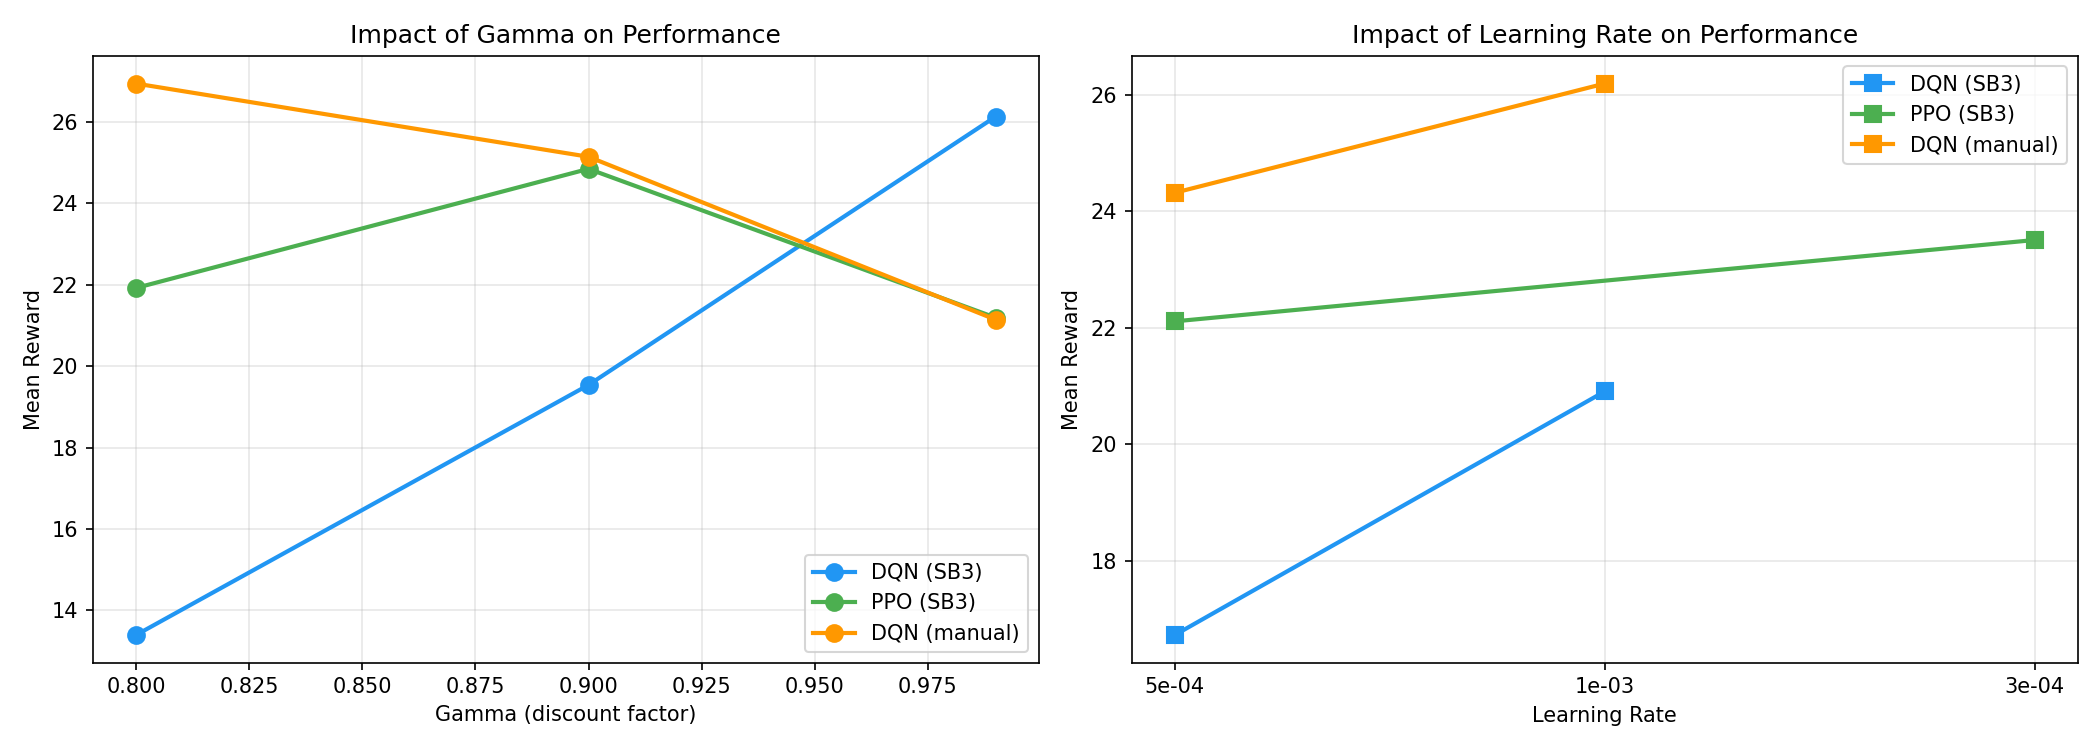
\includegraphics[width=\textwidth]{figures/hyperparam_exploration.png}
    \caption{Impact de $\gamma$ (gauche) et du learning rate (droite) sur la performance.}
    \label{fig:hyperparam}
\end{figure}

% ══════════════════════════════════════════════════
\section{Résultats et évolution par phases}

\subsection{Problèmes identifiés en Phase 2 (100k steps)}

L'entraînement à pleine puissance a révélé des problèmes majeurs~:

\begin{table}[H]
\centering
\begin{tabular}{l rrl}
\toprule
\textbf{Algo} & \textbf{Phase 2 final} & \textbf{Phase 2 best} & \textbf{Problème identifié}\\
\midrule
DQN SB3     & 12.92 & 23.98 (70k) & Q-value overestimation\\
PPO SB3     & 23.53 & 28.63 (35k) & Distribution shift on-policy\\
DQN Manual  & 19.73 & N/A         & Epsilon decay trop lent\\
\bottomrule
\end{tabular}
\caption{Résultats Phase 2 et problèmes diagnostiqués.}
\end{table}

\paragraph{DQN SB3 -- Q-value overestimation.}
Avec $\text{lr}=10^{-3}$ fixe, les Q-values sont surestimées à cause de l'opérateur $\max$ dans la cible $y = r + \gamma \cdot \max_{a'} Q_{\text{target}}(s', a')$. Le modèle passe de 23.98 (70k) à 12.92 (100k), soit $-46\%$.

\paragraph{PPO SB3 -- Distribution shift.}
Étant on-policy, quand la politique s'améliore, la distribution d'états change. Le clipping limite la chute ($-32\%$ vs $-46\%$ pour DQN) et permet un rebond partiel.

\paragraph{DQN Manual -- Bug epsilon decay.}
Configuré en gradient steps (15\,000), l'agent avait encore 62\% d'actions aléatoires à l'épisode 400. L'early stop se déclenchait car la reward d'entraînement (polluée par l'exploration) ne progressait plus, alors que la politique sous-jacente était potentiellement bonne.

\subsection{Corrections appliquées (Phases 3 et 4)}

\begin{table}[H]
\centering
\small
\begin{tabular}{llp{7cm}}
\toprule
\textbf{Algo} & \textbf{Correction} & \textbf{Impact}\\
\midrule
DQN SB3     & lr scheduler $10^{-3}\to 10^{-4}$ & Élimine l'effondrement post-pic\\
DQN SB3     & \texttt{target\_update}: $50\to 100$ & Ralentit la propagation des erreurs\\
\midrule
PPO SB3     & lr scheduler $3\!\times\!10^{-4}\to 3\!\times\!10^{-5}$ & Stabilise le training tardif\\
PPO SB3     & \texttt{n\_steps}: $256\to 512$, \texttt{ent\_coef}$=0.01$ & Gradients plus stables\\
PPO SB3     & Budget 80k + copie auto du best & Évite l'overtraining\\
\midrule
DQN Manual  & \texttt{epsilon\_decay}: $15\,000\to 5\,000$ & \textbf{Fix critique}~: $\varepsilon=0.05$ dès ép.~275\\
DQN Manual  & Eval déterministe périodique & Best model basé sur la vraie perf.\\
DQN Manual  & Gradient clipping (\texttt{max\_norm}$=10$) & Stabilise l'entraînement tardif\\
DQN Manual  & 1\,000 épisodes sans early stop & Exploitation complète\\
\bottomrule
\end{tabular}
\caption{Corrections ciblées par algorithme.}
\end{table}

\subsection{Résultats finaux}

\begin{table}[H]
\centering
\begin{tabular}{l rrrr}
\toprule
\textbf{Algo} & \textbf{Phase 1} & \textbf{Phase 2} & \textbf{Phase 3} & \textbf{Phase 4}\\
\midrule
DQN SB3     & 28.81 & 12.92 & \textbf{27.14} & 27.14\\
PPO SB3     & 26.08 & 23.53 & 21.92 & \textbf{27.88}\\
DQN Manual  & 28.46 & 19.73 & 8.35  & \textbf{27.54}\\
\bottomrule
\end{tabular}
\caption{Évolution des rewards moyennes à travers les 4 phases expérimentales.}
\label{tab:phases}
\end{table}

Les 3~algorithmes convergent vers $\sim$27--28 de reward en Phase~4. Malgré des architectures fondamentalement différentes, les 3~approches atteignent des performances similaires une fois correctement diagnostiquées et corrigées.

\begin{figure}[H]
    \centering
    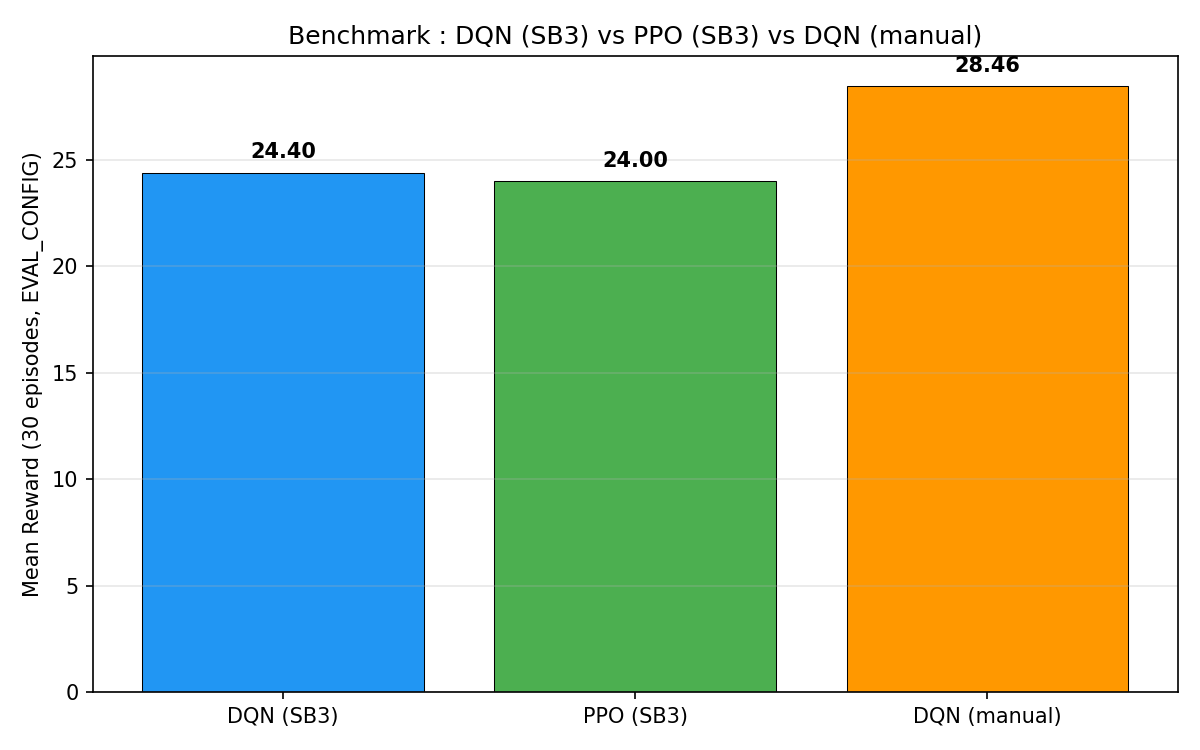
\includegraphics[width=0.75\textwidth]{figures/benchmark_comparison.png}
    \caption{Comparaison finale des 3 algorithmes (30~épisodes, \texttt{EVAL\_CONFIG}).}
    \label{fig:benchmark}
\end{figure}

% ══════════════════════════════════════════════════
\section{Analyse comparative}

\subsection{Benchmark final}

\begin{table}[H]
\centering
\begin{tabular}{l rrrr}
\toprule
\textbf{Algo} & \textbf{Reward} & \textbf{Std} & \textbf{Ep.~Length} & \textbf{Survie}\\
\midrule
\textbf{PPO SB3} & \textbf{27.88} & \textbf{4.80} & \textbf{38.2} & 95.5\%\\
DQN Manual        & 27.54          & 7.35          & 36.6          & 91.5\%\\
DQN SB3           & 27.14          & 8.17          & 34.8          & 87.0\%\\
\bottomrule
\end{tabular}
\caption{Benchmark final (30~épisodes, \texttt{EVAL\_CONFIG}).}
\label{tab:benchmark}
\end{table}

\textbf{PPO} est le meilleur modèle global~: meilleure reward, plus faible variance ($\sigma=4.80$), et meilleure survie (38.2/40~steps).

\subsection{Off-policy vs On-policy}

Le DQN (off-policy) réutilise les données du replay buffer, ce qui le rend plus sample-efficient en théorie mais moins stable (les données deviennent \emph{stale}). Le PPO (on-policy) jette les données après chaque update mais bénéficie de données toujours fraîches. Sur highway-env avec des véhicules agressifs (environnement hautement stochastique), la stabilité de PPO est un avantage significatif.

\subsection{SB3 vs implémentation manuelle}

Notre DQN manual est compétitif avec les modèles SB3 (27.54 vs 27.14 pour DQN SB3) malgré l'absence d'environnements vectorisés et d'optimisations ingénierie. Il est aussi nettement plus rapide à entraîner ($\sim$21~min pour 1\,000~épisodes vs $\sim$24~min pour 100k~steps SB3, grâce à l'absence d'overhead de logging et de vectorized env management).

\subsection{Courbe d'entraînement du DQN manual}

\begin{figure}[H]
    \centering
    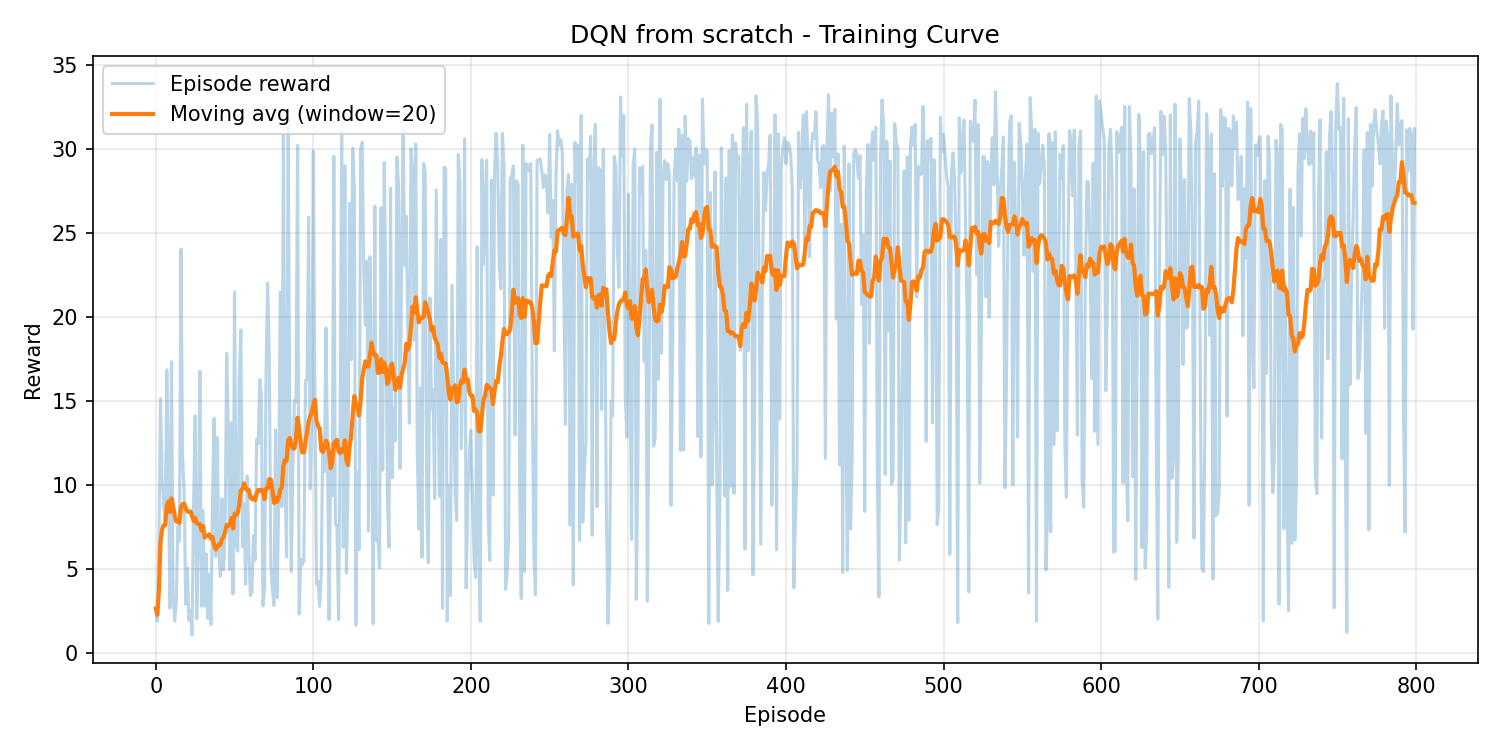
\includegraphics[width=0.85\textwidth]{figures/manual_dqn_training.png}
    \caption{Courbe d'entraînement du DQN manual~: exploration forte au début ($\varepsilon$ élevé), apprentissage rapide vers ép.~200--300, puis plateau en exploitation.}
    \label{fig:dqn_curve}
\end{figure}

% ══════════════════════════════════════════════════
\section{Overtraining et variance en RL}

\subsection{Le paradoxe de l'overtraining}

Contrairement au supervised learning où plus de données signifie un meilleur modèle, en RL le modèle \emph{génère ses propres données}. Une politique qui se dégrade produit des données de mauvaise qualité, créant un cercle vicieux. L'\texttt{EvalCallback} qui sauvegarde le best model est donc \textbf{indispensable}~: le modèle final (dernier step) n'est souvent pas le meilleur.

Nos résultats le démontrent clairement~: en Phase~2, les 3~algorithmes obtiennent des résultats inférieurs à la Phase~1 malgré un budget d'entraînement 3$\times$ supérieur. L'utilisation systématique de best checkpoints a été la clé pour récupérer les meilleures politiques.

\subsection{Variance inter-runs}

Le même algorithme avec les mêmes hyperparamètres peut donner des résultats très différents d'un run à l'autre, à cause de~:
\begin{enumerate}[nosep]
    \item \textbf{Seeds aléatoires}~: poids initiaux, ordre des transitions, épisodes rencontrés.
    \item \textbf{Environnement stochastique}~: véhicules à positions aléatoires, comportements variables.
    \item \textbf{Composition du replay buffer}~: différentes transitions mènent à des apprentissages différents.
    \item \textbf{Échantillonnage de l'évaluation}~: 15--30~épisodes restent un petit échantillon.
\end{enumerate}

Idéalement, il faudrait reporter des résultats moyennés sur 3--5~seeds. Le temps limité ne nous l'a pas permis, mais nous reconnaissons cette limite.

\subsection{L'approche itérative comme clé du succès}

Notre méthodologie \textbf{diagnostic $\to$ correction $\to$ retrain} a été la clé~: chaque phase a identifié des problèmes spécifiques (Q-value overestimation, epsilon trop lent, overtraining) et les corrections ciblées ont systématiquement fonctionné. Le DQN Manual est passé de 8.35 à 27.54 ($+230\%$) grâce à 5~corrections successives.

% ══════════════════════════════════════════════════
\section{Bonus~: Racetrack}

En bonus, nous avons appliqué nos algorithmes à l'environnement \texttt{racetrack-v0}, un circuit avec des virages serrés nécessitant des actions continues (accélération, direction). Nous avons utilisé~:
\begin{itemize}[nosep]
    \item \textbf{PPO (SB3)}~: adapté naturellement aux actions continues,
    \item \textbf{SAC (SB3)}~: Soft Actor-Critic, off-policy, spécialement conçu pour les espaces d'actions continus,
    \item \textbf{DQN manual}~: avec discrétisation de l'espace d'actions.
\end{itemize}

\begin{figure}[H]
    \centering
    \begin{subfigure}[t]{0.48\textwidth}
        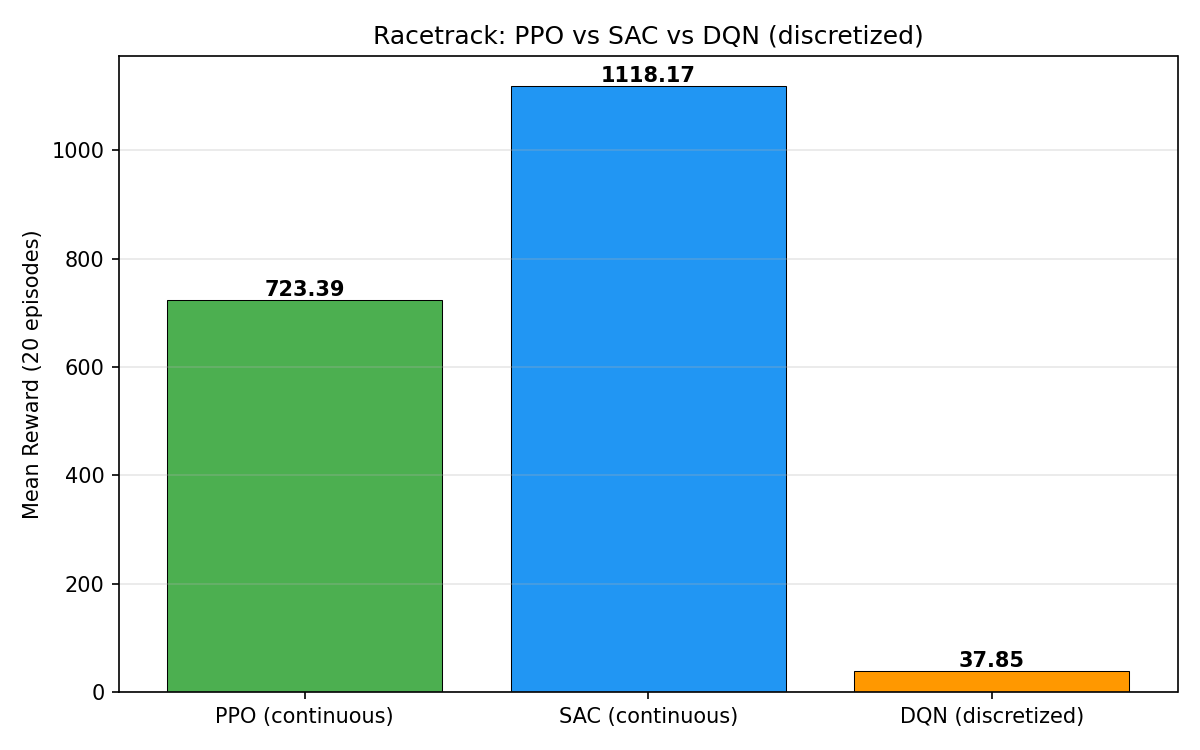
\includegraphics[width=\textwidth]{figures/racetrack_benchmark.png}
        \caption{Benchmark racetrack.}
    \end{subfigure}
    \hfill
    \begin{subfigure}[t]{0.48\textwidth}
        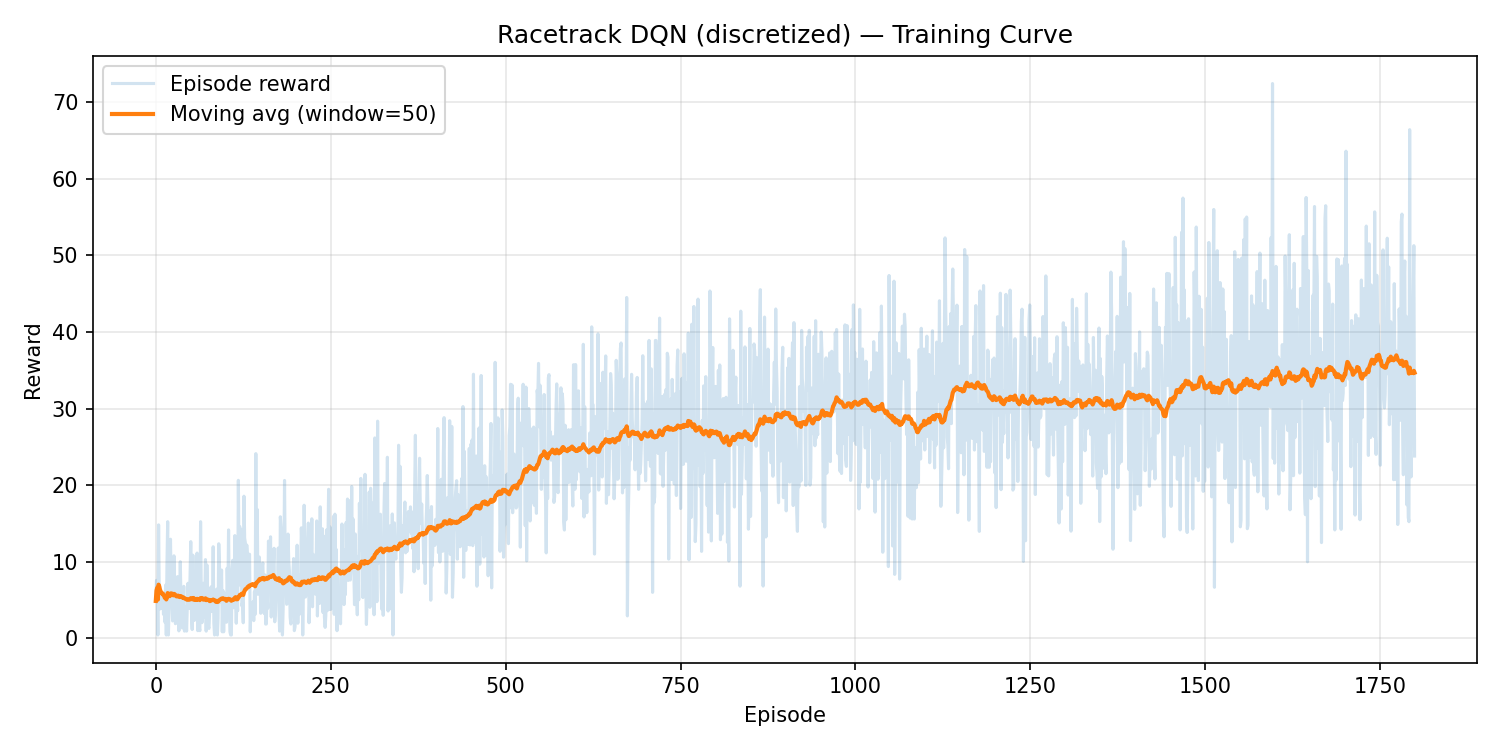
\includegraphics[width=\textwidth]{figures/racetrack_dqn_training.png}
        \caption{Courbe d'entraînement DQN.}
    \end{subfigure}
    \caption{Résultats sur l'environnement racetrack (bonus).}
    \label{fig:racetrack}
\end{figure}

Le SAC (off-policy, actions continues) s'avère particulièrement adapté à ce type d'environnement, tandis que le PPO reste compétitif.

% ══════════════════════════════════════════════════
\section{Conclusion}

Ce projet nous a permis de mettre en pratique les concepts fondamentaux du RL~:
\begin{itemize}[nosep]
    \item \textbf{DQN}~: comprendre le replay buffer, le target network, et le problème de Q-value overestimation.
    \item \textbf{PPO}~: comprendre l'approche actor-critic, le clipping, et le trade-off on/off-policy.
    \item \textbf{Implémentation manuelle}~: maîtriser chaque composant du DQN (réseau, buffer, epsilon-greedy, boucle d'entraînement).
    \item \textbf{Tuning}~: l'importance cruciale des hyperparamètres ($\gamma$, lr) et des techniques de stabilisation (lr schedulers, gradient clipping, EvalCallback).
\end{itemize}

Le principal enseignement est que le RL est un domaine où l'\textbf{ingénierie expérimentale} compte autant que la théorie~: diagnostiquer les problèmes, proposer des corrections ciblées, et valider itérativement est essentiel pour obtenir de bonnes performances.

% ══════════════════════════════════════════════════
\newpage
\begin{thebibliography}{9}

\bibitem{mnih2015}
V.~Mnih et al., \emph{Human-level control through deep reinforcement learning}, Nature, vol.~518, pp.~529--533, 2015.

\bibitem{schulman2017}
J.~Schulman, F.~Wolski, P.~Dhariwal, A.~Radford, O.~Klimov, \emph{Proximal Policy Optimization Algorithms}, arXiv:1707.06347, 2017.

\bibitem{vanhasselt2016}
H.~van Hasselt, A.~Guez, D.~Silver, \emph{Deep Reinforcement Learning with Double Q-learning}, AAAI, 2016.

\bibitem{highwayenv}
E.~Leurent, \emph{An Environment for Autonomous Driving Decision-Making}, \url{https://github.com/Farama-Foundation/HighwayEnv}, 2018.

\bibitem{sb3}
A.~Raffin et al., \emph{Stable-Baselines3: Reliable Reinforcement Learning Implementations}, JMLR, vol.~22, no.~268, pp.~1--8, 2021.

\end{thebibliography}

% ══════════════════════════════════════════════════
\newpage
\appendix
\section{Structure du code}

\begin{table}[H]
\centering
\begin{tabular}{lp{9cm}}
\toprule
\textbf{Fichier} & \textbf{Description}\\
\midrule
\texttt{Final\_Project.ipynb} & Notebook principal (entraînement, évaluation, figures)\\
\texttt{Final\_Project.py} & Version Python du notebook (format percent)\\
\texttt{models/} & Poids des modèles entraînés (\texttt{.zip} SB3, \texttt{.pt} PyTorch)\\
\texttt{figures/} & Graphiques de benchmark et hyperparamètres\\
\texttt{videos/} & Vidéos de l'agent aléatoire et entraîné\\
\texttt{bonus/} & Environnement racetrack (notebook, modèles, figures)\\
\texttt{trainv2.py}, \texttt{trainv3.py} & Scripts d'entraînement (Phases 3 et 4)\\
\bottomrule
\end{tabular}
\caption{Structure du dépôt.}
\end{table}

\end{document}
